\documentclass[UKenglish, unknownkeysallowed]{beamer}


% Change the overall appearance by choosing a different theme.
% Possible standard values:
% default, AnnArbor, Antibes, Bergen, Berkeley, Berlin, Boadilla, CambridgeUs,
% Copenhagen, Darmstadt, Goettingen, PaloAlto, Szeged, Warsay
\usetheme{Madrid}


% Change just the color by choosing a different color theme.
% Possible standard values:
% default, beaver, beetle, seahorse, wolverine
\usecolortheme{beaver}


% If the MathDept theme is downloaded,
% you can replace the above two lines with:
%\usetheme{MathDept}


% Compare the frames about overlays with and without this option:
%\setbeamercovered{transparent}


\usepackage[utf8]{inputenx}
\usepackage{babel}
\usepackage[final]{microtype}
\usepackage{textcomp}
\usepackage{listings}


\usepackage{tikz}
\usetikzlibrary{mindmap}
\usetikzlibrary{overlay-beamer-styles}  % Overlays for TikZ
\usepackage[absolute, overlay]{textpos} % Arbitrary positioning
\setlength{\TPHorizModule}{\paperwidth} % Textpos units
\setlength{\TPVertModule}{\paperheight} % Textpos units
\usepackage{multimedia}                 % Include media files


% The below macros have an optional argument to shorten the content.
% Typically, the long version is printed on the title frame
% and the short version is printed on the ordinary frames.
% This depends on the Beamer theme.
\author[Helsø]{Martin Helsø}
\title[Beamer]{Introduction to Beamer}
\subtitle[Project work]{MAT2000, MEK3200, STK-MAT2011}
\institute[UiO]{University of Oslo}
\date[\the\day.\the\month.\the\year]{\today} % Really unnecessary abbreviation


\begin{document}


% Remove this frame if using the theme MathDept:
\begin{frame}[plain, noframenumbering]
    \titlepage
\end{frame}


\section{Colours}


\begin{frame}
    \frametitle{Colours}

    \begin{itemize}
        \item
        Most Beamer themes are designed around a single colour called the \structure{structure colour}.

        \item
        Do not use \emph{emph} to highlight something.
        Use \alert{alert}.
        Normally,
        \alert{alert} changes the text colour into something bright and highly visible,
        but it can be configured to modify the font further.

        \item
        You can of course use \textcolor{green}{any colour}, as usual.
    \end{itemize}

    The above three colour commands are compatible with overlays,
    which we will come back to.
\end{frame}


\section{Layout}
\subsection{Blocks}


\begin{frame}
    \frametitle{Blocks}

    \begin{block}{Basic Block}
        One common way to divide the text is to use blocks.
    \end{block}

    \begin{exampleblock}{Example Block}
        They come in three types, for variation and \alert{highlighting}.
    \end{exampleblock}

    \begin{alertblock}{Alert Block}
        Apart from \alert{alertblock},
        blocks are typically not used directly like this\ldots
    \end{alertblock}

    \begin{theorem}
         \ldots but via some environment.
    \end{theorem}
\end{frame}


\subsection{Columns}


\begin{frame}
    \frametitle{Columns}

    \begin{columns}[onlytextwidth]
        \begin{column}{0.49\textwidth}
            Another way to divide the text is by the use of \alert{columns}.

            \begin{example}
                This can easily be combined with \alert{blocks}.
            \end{example}

            \begin{enumerate}
                \item
                And with \alert{lists}.
            \end{enumerate}
        \end{column}

        \begin{column}{0.49\textwidth}
            Note that the textwidth is locally redefined to equal the width of the column:
            \begin{center}
                
\includegraphics[width = 0.8\textwidth]{apollon}
            \end{center}
        \end{column}
    \end{columns}
\end{frame}


\subsection{Textpos}


\begin{frame}[fragile]
    \frametitle{Textpos}

    There is no reason to use floats in a Beamer,
    as pictures and tables shall stay within the frame.
    There is also no need for captions,
    as you will explain the figure orally.
    Normally, we let \LaTeX\ decide where objects should be placed,
    but here we want complete control.
    This is attained with the \alert{textpos} package.

    \medskip

    The syntax for textpos is as follows:

\begin{lstlisting}[language = {[LaTeX]{TeX}}]
\begin{textblock}{<width>}(x, y)
    <content>
\end{textblock}
\end{lstlisting}

    This creates a box with the specified width and upper left corner at the point (x, y).
    For this document, I have set the units to be paperwidth and paperheight.
    The box can be filled with anything.
\end{frame}


\begin{frame}
    \frametitle{Textpos \textthreequartersemdash\ Example}

    \begin{textblock}{0.3}(0.25, 0.22)
        
\includegraphics[width = \textwidth]{apollon}
    \end{textblock}

    \begin{textblock}{0.3}(0.6, 0.05)
        
\includegraphics[width = \textwidth]{apollon}
    \end{textblock}

    \begin{textblock}{0.2}(0.1, 0.6)
        
\includegraphics[width = \textwidth]{apollon}
    \end{textblock}
\end{frame}


\section{Overlays}


\begin{frame}
    \frametitle{Overlays}

    We can control when objects appear on the frame with \alert{overlays}.

    \pause
    \medskip

    The simplest overlay command is \alert{pause}.
    If you pause somewhere in a frame,
    only the text up until the first pause is showed on the first slide.
    On the second slide, everything is shown up to the second pause, and so forth.

    \pause
    \medskip
    There are more flexible commands:

    \begin{description}
        \item[onslide]
        displays text only on specified slides.
        The text occupies space when hidden.

        \item[only]
        displays text only on specified slides.
        The text occupies no space when hidden.

        \item[alt]
        displays one text on specified slides and another text on the rest of the slides.
    \end{description}

    Here `text' also includes other objects, such as images.
\end{frame}


\subsection{Examples}


\begin{frame}
    \frametitle{Overlays \textthreequartersemdash\ Examples}

    % We specify slides within <>.
    % It can either be a list of slides, such as <1> or <1, 3, 5>
    % Or a range, such as <-3>, <3-5> or <2->
    % Or a combination, such as <1, 3-5>

    This text is shown on all slides.
    \onslide<2>{\alert{This text is only shown on the second slide.}}
    This text is shown on all slides.

    \medskip

    This text is shown on all slides.
    \only<3>{\alert{This text is only shown on the third slide.}}
    This text is shown on all slides.

    \medskip

    \alt<1,3>{This text is shown on the first and third slide.}
             {\alert{This text is shown on the second slide.}}
\end{frame}


\begin{frame}
    \frametitle{Overlays \textthreequartersemdash\ Further Examples}

    The same \structure<1>{syntax} can be used
    for many \alert<2>{common} \textcolor<1>{green}{macros}
    and \textbf<2>{environments}.

    \begin{lemma}<2->[Zorn]
        Suppose a partially ordered set \(P\) has the property
        that every chain has an upper bound in \(P\).
        Then the set \(P\) contains at least one maximal element.
    \end{lemma}

    The latter takes up space when it is hidden.

    \begin{enumerate}
        \item<1->
        This is the first list item.

        \item<2->
        This is the second list item.

        \item<1->
        This is the third list item.
    \end{enumerate}
\end{frame}


\subsection{Lists}


\begin{frame}
    \frametitle{Overlays \textthreequartersemdash\ Lists}

    For lists, there is a special syntax for adding a pause between each item:

    \begin{itemize}[<+->]
        \item
        This is the first list item.

        \item
        This is the second list item.

        \item
        This is the third list item.
    \end{itemize}

    \pause
    We can take this one step further and highlight the last revealed item:

    \begin{itemize}[<+-| alert@+>]
        \item
        Cusp

        \item
        Node

        \item
        Triple point

        \item
        Quadruple point
    \end{itemize}

    % This combines nicely with other overlays:
    \only<5>
    {
        \begin{textblock}{0.15}(0.5, 0.6)
            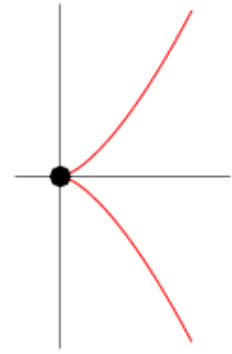
\includegraphics[width = \textwidth]{cusp}
        \end{textblock}
    }

    \only<6>
    {
        \begin{textblock}{0.15}(0.5, 0.6)
            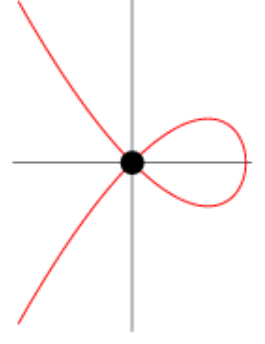
\includegraphics[width = \textwidth]{node}
        \end{textblock}
    }

    \only<7>
    {
        \begin{textblock}{0.25}(0.5, 0.6)
            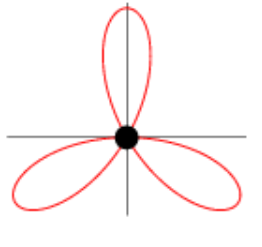
\includegraphics[width = \textwidth]{triple}
        \end{textblock}
    }

    \only<8->
    {
        \begin{textblock}{0.2}(0.5, 0.6)
            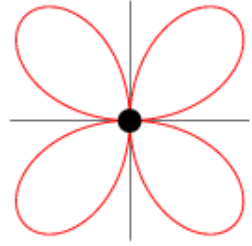
\includegraphics[width = \textwidth]{quadruple}
        \end{textblock}
    }
\end{frame}


\subsection{TikZ}


\begin{frame}
    \frametitle{Overlays \textthreequartersemdash\ Ti\textit{k}Z}

    While you can use pause, onslide, only and alt in Ti\textit{k}Z,
    this is often buggy.
    Instead, use the library \alert{overlay-beamer-styles},
    which provides tags such as `visible on', `draw on' and `fill on'.
    These can take overlay specifications:

    \centering
    \begin{tikzpicture}[mindmap, concept color = structure, text = white]

        \tikzstyle{level 1 concept}+=[sibling angle = 90, level distance = 25mm]

        \node[concept, scale = 0.6]{Main concept}
            [clockwise from = 135]
            child[concept color = alert, visible on = <2->]
                { node[concept, scale = 0.6]{Linked idea} }
            child[concept color = alert, visible on = <3->]
                { node[concept, scale = 0.6]{Association} }
            child[concept color = alert, visible on = <4->]
                { node[concept, scale = 0.6]{Mental connection} }
            child[concept color = alert, visible on = <5->]
                { node[concept, scale = 0.6]{Connotation} };
    \end{tikzpicture}
\end{frame}


\subsection{Handout Mode}


\begin{frame}[fragile]
    \frametitle{Disable Overlays}

    You can remove all overlay effects with the document class option \alert{handout}:
\begin{lstlisting}[language = {[LaTeX]{TeX}}]
\documentclass[handout]{beamer}
\end{lstlisting}
    This collapses all slides in a frame to a single slide.
\end{frame}


\section{Animations and Sound}


\begin{frame}
    \frametitle{Animations and Sound}

    It is easy to include animations and sound in Beamer.
    Simply use the \alert{multimedia} package
    and \alert{movie} command (even for sound files!).
    The difficulty is finding a PDF viewer capable of playing the media file.
    Acrobat Reader 6 on MacOS can play anything that QuickTime can play.
    In Linux, you can play media files with Okular
    if you compile with the document class option \structure{unknownkeysallowed}.

    \medskip

    If the PDF viewer is capable of playing the media file,
    then you can use the options \alert{autostart} or \alert{loop}
    with the \alert{movie} command.

    \medskip

    Otherwise, use the option \alert{externalviewer}
    in order to open another viewer to play the file.

    \medskip

    The media file must lie in the same folder as the PDF.
\end{frame}


\subsection{Example}


\begin{frame}
    \frametitle{Animations and Sound \textthreequartersemdash\ Example}

    Check if your PDF viewer can play \texttt{.mp4} by clicking the picture.

    \begin{center}
        \movie{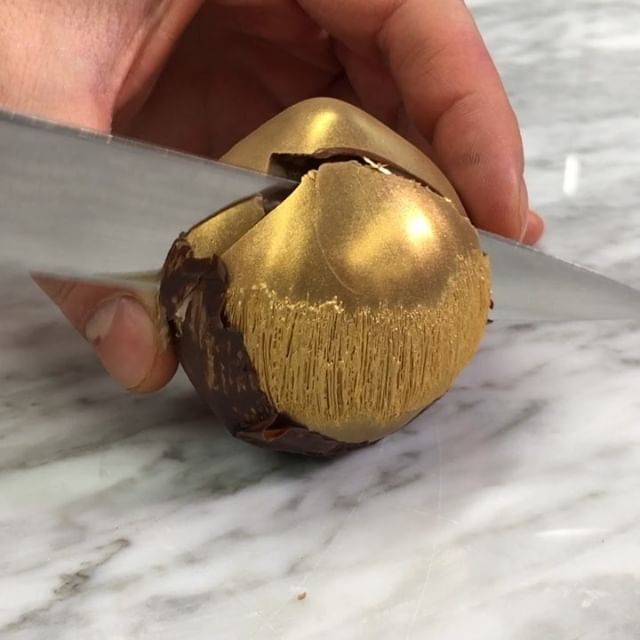
\includegraphics[scale = 0.2]{hazelnut-still}}{hazelnut.mp4}
    \end{center}

    If it cannot, \movie[externalviewer]{\alert{click here}}{hazelnut.mp4}.
\end{frame}


\section{Frame Options}


\begin{frame}
    \frametitle{Frame Options}

    \begin{description}
        \item[plain]
        removes the header and footer.
        Use this if you need extra space,
        for instance if displaying a full-frame picture.

        \item[fragile]
        tells Beamer that the frame contains text that is not interpreted the way that text is usually interpreted by \TeX.
        In particular, use this if the frame contains verbatim text, such as code.

        \item[allowframebreaks]
        automatically splits the frame into several frames if the content exceeds a single frame.
        The drawback is that overlays cannot be used with this option in effect.
        Hence, reserve this option for a long bibliography.
    \end{description}
\end{frame}


\subsection{Plain Example}


\begin{frame}[plain]
    \begin{textblock}{1}(0, 0)
        \centering
        
\includegraphics[height = \paperheight]{apollon}
    \end{textblock}
\end{frame}


\section{Posters}


\begin{frame}
    \frametitle{Posters}

    You can easily create posters with Beamer.
    All you need is the package \alert{beamerposter}.
    The package provides options for selecting paper size, orientation and a scale factor for fonts.
    The poster itself consists of a single Beamer frame with no overlays.
\end{frame}


\section{Bibliography}


\begin{frame}
    \frametitle{Bibliography}

    A bibliography is neither necessary nor recommended in a presentation.
    It should be written manually and contain less information
    than a bibliography found in a research paper.

    \begin{thebibliography}{}

        % Icon
        \setbeamertemplate{bibliography item}[book]

        \bibitem{Har77}
        R.~Hartshorne
        \newblock Algebraic Geometry
        \newblock Springer-Verlag, 1977

        % Icon
        \setbeamertemplate{bibliography item}[online]

        \bibitem{Hel17}
        M.~Helsø
        \newblock Rational Quartic Symmetroids, 2017
        \newblock \url{https://arxiv.org/abs/1708.04101}

        % Icon
        \setbeamertemplate{bibliography item}[article]

        \bibitem{Ott+14}
        J.~C.~Ottem et al.
        \newblock Quartic spectrahedra
        \newblock Mathematical Programming, 2014

    \end{thebibliography}
\end{frame}


\end{document}